\documentclass{article}
\usepackage{graphicx}
\usepackage{url}
\usepackage{indentfirst}
\usepackage{float}


\begin{document}

\title{Market Study for Digital Wallets}
\maketitle

\section{Introduction}

In recent years, digital wallets have emerged as a dominant trend, providing users with the convenience of carrying and using their payment cards, along with a variety of other documents, such as ID cards and transportation tickets, in a completely digital way. By storing these documents securely and encrypted, these applications not only offer convenience, but also guarantee the security of users' sensitive data.

Additionally, digital wallets constitute a greener and more sustainable approach, as they reduce the need for physical cards and paper, contributing to the preservation of the environment.

Given our lack of prior knowledge, we decided to carry out an in-depth study of the market to identify the best possible approach. In this regard, we analyzed various applications that use technologies such as NFC (Near Field Communication), digital wallets and other projects from other universities that have also migrated from physical cards to virtual cards. This comprehensive research allowed us to gain valuable knowledge about current trends and effective practices, providing a solid basis for the design and implementation of our own project.

\section{NFC}

NFC is a technology that allows the exchange of information between compatible devices over a very short distance, usually up to 4cm. Devices with this technology, when placed close together, are able to create a radio frequency field that enables them to communicate.

\subsection{Main modes of operation}
\begin{itemize}
    \item \textbf{Reader/Writer mode: } In this mode, the NFC device functions as a reader that can interact with passive NFC tags (such as cards or labels) to read or write information on them. This mode is used for contactless payments, access to facilities, etc...
    \item \textbf{Card Emulation Mode: } In this mode, the NFC device works as if it were an NFC card, allowing it to be detected and read by other devices, such as payment terminals or facility access readers;
    \item \textbf{Peer-to-Peer mode: } In this mode, two NFC devices can exchange information bidirectionally. This allows direct communication between the devices, facilitating data transfer, such as file exchange, information sharing or even mobile payments between the devices.
\end{itemize}

Of the existing operating modes, Card Emulation Mode is particularly relevant, as it allows mobile devices to act as
as university cards, facilitating access to university services and facilities, and even use
even use for digital student identification. It also allows for payments, something that should be possible with our cards.
In order to better understand how to implement these modes, we decided to analyze in which situations NFC is used and in which cases it is most effective:

\begin{itemize}
    \item \textbf{MB Way:} A mobile payment application that allows you to carry out various transactions using your cell phone. It uses NFC to make payments in physical stores, so all you have to do is bring your phone close to the scanning terminal.
    \item \textbf{Digital Mobile Key:} A digital authentication application that allows Portuguese citizens to access various online services with their cell phone. It uses NFC to authenticate the user in online services, simply by bringing the cell phone close to the reader terminal.
    \item \textbf{App Anda:} An application for paying journeys on public transport in the Porto Metropolitan Area. It uses NFC to pay for journeys, simply by bringing the card close to the validator.
\end{itemize}


\section{Digital Wallets}

Digital wallets are virtual platforms that allow users to store and manage financial and personal information electronically. They facilitate payments online and in physical stores, offering convenience and security. Digital wallets are becoming popular due to the convenience of storing multiple cards and the additional protection against fraud.

\subsection{Use Cases}

\begin{itemize}
    \item \textbf{University card:} Users can use their virtual card as if it were their physical card, speeding up the process of using university services;
    \item \textbf{Payments in physical stores:} Users can pay for their purchases in physical stores, using their virtual payment cards and avoiding the use of physical cards;
    \item \textbf{Identification:} The user can use their digital wallet to identify themselves when necessary;
    \item \textbf{Transport tickets:} The user can have a virtual transport pass, just like a transport ticket, avoiding the need to have a physical ticket;
\end{itemize}


Our application will be a digital wallet that will focus on the use cases of a university card and identification. Despite this, it won't differ much from other applications that use digital wallets for other purposes, so these can be used as examples. In order to develop a good implementation of a digital wallet, we analyzed some existing applications.

\subsection{Apple Wallet}
Apple Wallet is one of the most popular digital wallets. You can use it on Apple products other than your cell phone, such as the Apple Watch and iPad. In addition to the possibility of adding payment cards, Apple Wallet allows you to use Apple Pay, Apple's payment service that makes it easy to make payments in physical stores and online. However, this digital wallet is integrated with many other services that allow users to add loyalty cards, transport tickets and more.

In order to guarantee security for its users, cards such as loyalty cards, identification documents, among others, need a trusted certificate to be added to the digital wallet, ensuring that they are genuine.
Although payment cards in the Apple wallet also need to guarantee their eligibility, in these cards, the Apple wallet communicates with the card provider, guaranteeing the legitimacy of the card and users authenticate themselves to ensure that they are the owners of the card. To minimize the risk of compromised information theft, a unique token, which stores the card information, is generated and encrypted on the device's Secure Element Chip, ensuring that the card information is not shared.

\begin{figure}[H]
    \centering
    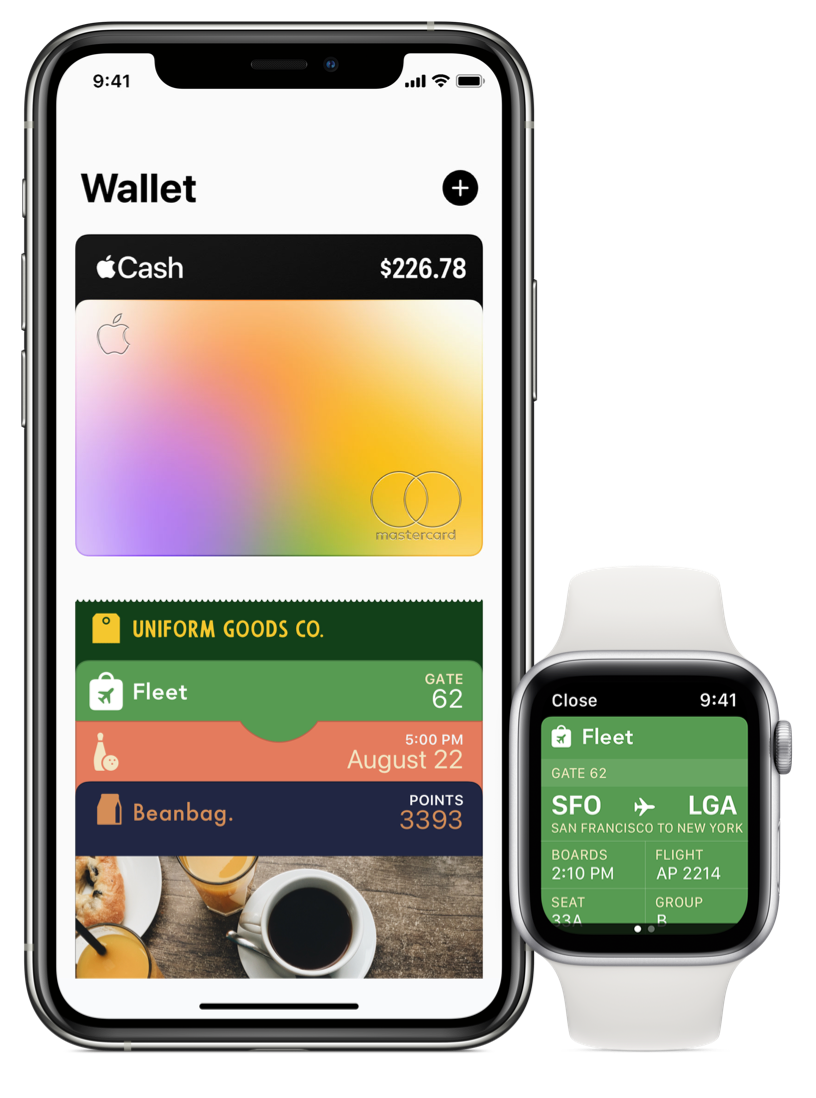
\includegraphics[width=0.5\textwidth]{images/Apple_Wallet.png}
    \caption{Graphic interface of Apple Wallet}
    \label{fig:my_label}
\end{figure}

\subsection{Google Wallet}
Like Apple Wallet, Google Wallet is one of the most popular digital wallets. Like the previous one, it allows you to add different types of cards and can be used on devices other than just cell phones. In addition, Google Wallet allows the use of Google Pay, a service that guarantees the user the possibility of making payments.
In order to certify the eligibility of the cards it adds, Google Wallet needs the card providers to have used a legitimate certificate. In the case of cards used for payments, Google Wallet communicates with the user's bank and verifies their identity through user authentication. As with Apple Wallet, in order to guarantee the security of payment card information, a unique token is used that encrypts the card information.

\begin{figure}[H]
    \centering
    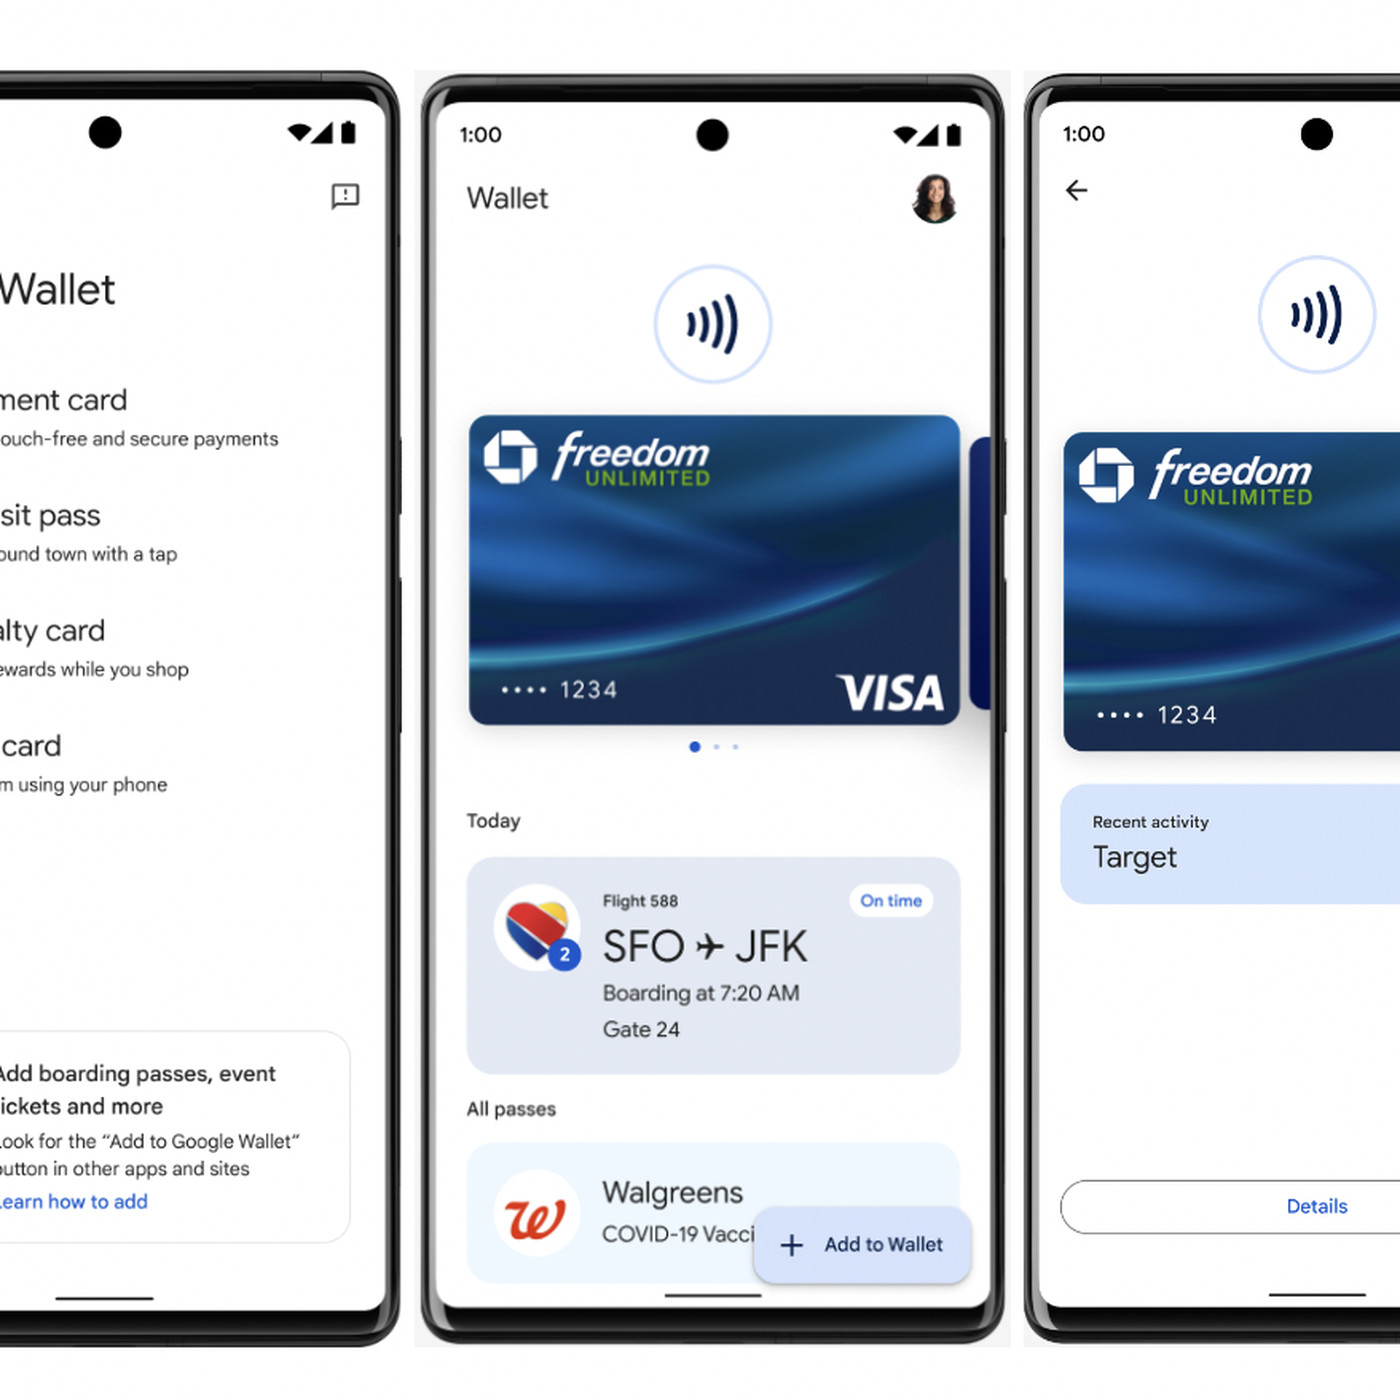
\includegraphics[width=0.5\textwidth]{images/Google_Wallet.png}
    \caption{Graphic interface of Google Wallet}
    \label{fig:my_label}
\end{figure}

\section{Panorama of the Education and University Market}
As part of a preliminary study into the higher education sector, we have dedicated ourselves to exploring the current state of innovation, with particular attention to the institutions
that have already implemented the virtual student card. This interest stems from the
growing trend towards the digitization of academic services, with the aim of both
optimizing processes and improving the student experience.

\subsection{International Adoption of Digital Student Cards}
Google Wallet already facilitates the use of digital student cards at
several colleges located in Australia, the United States and Canada, indicating
a significant advance in the adoption of this technology on a global scale. Among the
pioneering institutions in this initiative are:

\begin{itemize}
    \item \textbf{Monash University, Australia: }Monash University stands out for its
          innovation with M-Pass, which integrates with Google Wallet and Apple Wallet.
          This system not only reflects adaptability to emerging technological
          trends, but also highlights the potential for transforming academic
          academic services through digitalization. The acquisition of M-Pass requires
          that students authenticate themselves with their academic credentials and
          validate their identity by submitting an official document (passport or driver's license). This process emphasizes security and
          authentication, which are fundamental to the success of such digital initiatives.
          Through the university's app, students can load credits
          to the card, although the full functionality of the card has not been
          fully specified.
    \item \textbf{University of York, Canada: }The YU-Card, implemented by the University of
          York, provides students with a practical way to access a wide range of
          university services and spaces. Unlike the M-Pass,
          the YU-Card is rechargeable via the university's website.
\end{itemize}

\subsection{European Perspectives}
In Europe, the European Student Card (ESC) initiative is set to offer a digital solution to higher education institutions participating in the Erasmus+ program by 2025. This initiative underscores a dedication to enhancing student mobility and integrating academic services through digital platforms. It represents a significant move towards the harmonization and streamlining of educational processes across Europe, facilitating a more unified and simplified academic experience for students.


% Here you can write a conclusion about your market analysis.
\begin{thebibliography}{9}
    \bibitem{ApplePaycomponentsecurity}
    \textit{Apple Pay Component Security},
    \url{https://support.apple.com/guide/security/apple-pay-component-security-sec2561eb018/web}

    \bibitem{applewallet}
    \textit{Apple Wallet},
    \url{https://developer.apple.com/wallet/get-started/}

    \bibitem{applepay}
    \textit{Apple Pay},
    \url{https://support.apple.com/en-us/HT203027}

    \bibitem{genericPass}
    \textit{Generic Cards},
    \url{https://developers.google.com/wallet/generic}

    \bibitem{googlewallet}
    \textit{Google Wallet},
    \url{https://wallet.google/}

    \bibitem{googlepay}
    \textit{Google Pay},
    \url{https://developers.google.com/pay/issuers/tsp-integration/overview}

    \bibitem{monash}
    \textit{Monash University},
    \url{https://www.monash.edu/students/support/connect/id}

    \bibitem{york}
    \textit{York University},
    \url{https://www.yorku.ca/yucard/}

    \bibitem{esc}
    \textit{European Student Card},
    \url{https://erasmus-plus.ec.europa.eu/european-student-card-initiative/card/about}

    \bibitem{campusMobileWallet}
    \textit{Campus Mobile Wallet},
    \url{https://en.wikipedia.org/wiki/List_of_campus_identifications_in_mobile_wallets}

\end{thebibliography}
\end{document}